\chapter{SAP}
\label{Kapitel:Einleitung}

SAP NetWeaver Business Intelligence (kurz: SAP BI) (vormals: Business Information Warehouse, kurz BW) ist die Data-Warehouse-Anwendung (kurz DW) der SAP AG und Teil von SAP NetWeaver. BW besteht unter anderem aus Komponenten zum Datenmanagement (Data Warehousing Workbench), zur Definition von Benutzerabfragen über einen OLAP-Prozessor (Business Explorer, kurz BEx), aus einer Data-Mining-Umgebung (Analyseprozessdesigner, kurz APD) und einer Komponente zur Kontrolle der Ladeprozesse. Die derzeitige Version des SAP Business Intelligence hat die Releasenummer 7.3 und ist Teil des SAP NetWeaver 7.3. 
Q: \url{http://de.wikipedia.org/wiki/SAP_NetWeaver_Business_Intelligence}


\section{Unterkapitel}
\label{Abschnitt:Motivation}

\begin{figure}[H]
    \centering
    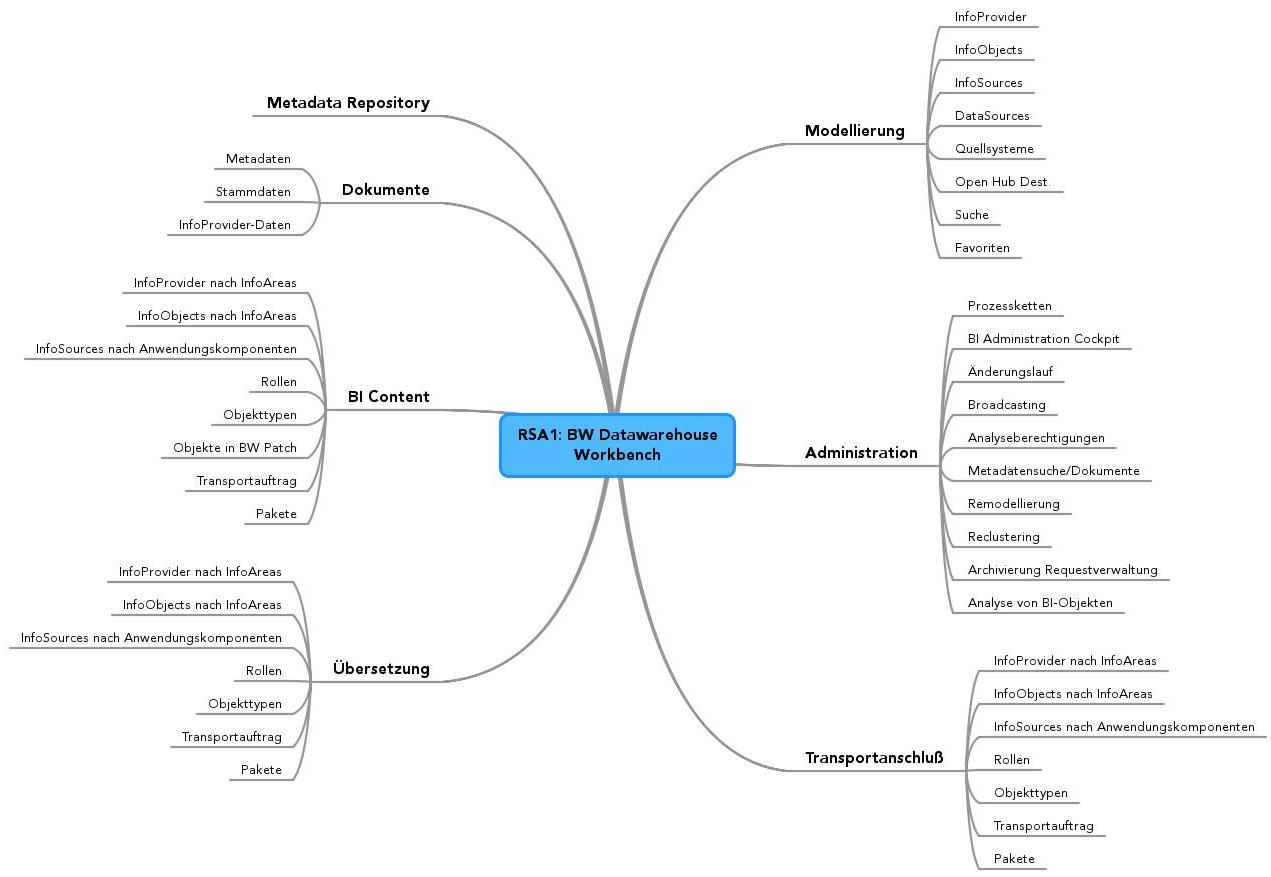
\includegraphics[width=1\textwidth]{files/RSA1Mindmap}
    \caption{Übersicht über RSA1}
    \label{pic:DWOverview}
\end{figure}


Die \textit{ Data Warehousing Workbench} lässt sich in die folgenden sieben Module unterteilen:\\


\begin{description}
\item[Modellierung:] Dieses Modul dient zur Modellierung von Daten und es werden verschiedene BI-Objekte bereitgestellt, welche zur Integration, Transformation, Konsolidierung, Bereinigung und Ablage von Daten genutzt werden können. Die verfügbaren BI-Objekte sind folgende:
\begin{itemize}
\item InfoProvider
\item InfoObjects
\item InfoSources
\item DataSources
\item Quellsysteme
\end{itemize}
Die Grafische Oberfläche ist in Abb. x zu sehen.
\begin{figure}[H]
    \centering
    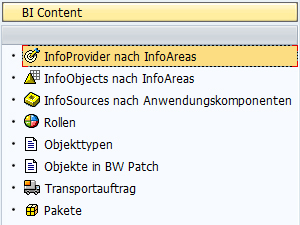
\includegraphics[width=0.5\textwidth]{files/BIContent}
    \caption{Das Modellierungsmenü}
    \label{pic:DWOverview}
\end{figure}
\item[Administration:] Hier befindet sich eine Ansicht für die verschiedensten Prozessketten, sowie das BI Administration Cockpit. Jenes wird verwendet, um die Performance von BI-Systemen zu überwachen. Es liefert einen zentralen Einstiegspunkt, sowie ein real-Time Monitoring und verschiedene Laufzeitstatistiken. Es bietet Zugriff auf Berichte und Anwendungen, die den Anwender bei der Ermittlung und Analyse von Problemen unterstützt. Es können BI-Objekte nachverfolgt und die Performance von BI-Aktivitäten optimiert werden.
Die Grafische Oberfläche ist in Abb. x zu sehen.
\begin{figure}[H]
    \centering
    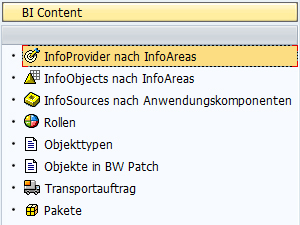
\includegraphics[width=0.5\textwidth]{files/BIContent}
    \caption{Das Administrationsmenü}
    \label{pic:DWOverview}
\end{figure}
\item[BI Content:] Die Struktur der verarbeiteten Geschäftsinformationen eines Unternehmens kann zu Auswertungszwecken im BI Content modelliert werden. Diese Modelle setzen sich aus verschiedenen Metadaten-Objekttypen zusammen. Hierbei werden vorkonfigurierte zur Analyse betriebswirtschaftlicher Fragestellungen verwendet. Wichtig hierbei ist, dass die Erzeugung, Verwendung, Überarbeitung und der Transport der BI-Objekte konsistent gehalten wird. Ein enthaltenes Konzept ist das \textit{BI-Versionskonzept} und eine Hauptfunktionalität ist die Übernahme von neuem BI Content in das Produktivsystem.
Die Grafische Oberfläche ist in Abb. x zu sehen.
\begin{figure}[H]
    \centering
    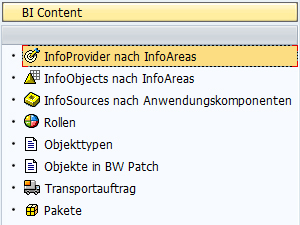
\includegraphics[width=0.5\textwidth]{files/BIContent}
    \caption{das BI Content Menü}
    \label{pic:DWOverview}
\end{figure}
\item[Transportanschluss:] Hier werden die selben Funktionalitäten wie in dem Modul \textit{BI Content} unterstützt, es besteht allerdings noch zusätzlich die Möglichkeit, BI-Objekte im XML-Format zu importieren bzw. zu exportieren.
Die Grafische Oberfläche ist in Abb. x zu sehen.
\begin{figure}[H]
    \centering
    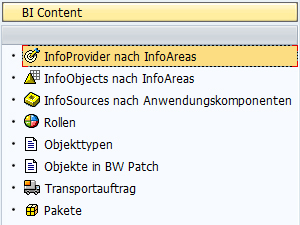
\includegraphics[width=0.5\textwidth]{files/BIContent}
    \caption{Übersicht über RSA1}
    \label{pic:DWOverview}
\end{figure}
\item[Dokumente:] Zu jedem BI-Objekt können jeweils ein oder mehrere Dokumente in verschiedenen Formaten, Versionen und Sprachen hinzugefügt, verlinkt und durchsucht werden. Diese Dokumente sind in drei Klassen unterteilt und können jeweils \textit{Metadaten}, \textit{Stammdaten} oder \textit{InfoProvider-Daten} zugeordnet werden.
Die Grafische Oberfläche ist in Abb. x zu sehen.
\begin{figure}[H]
    \centering
    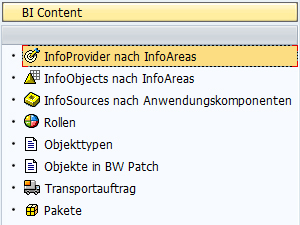
\includegraphics[width=0.5\textwidth]{files/BIContent}
    \caption{Das Dokumente Menü}
    \label{pic:DWOverview}
\end{figure}
\item[Übersetzung:] Um eine Internationalisierung umsetzen zu können, können mit Hilfe des Moduls \textit{Übersetzung} die Kurz- und Langtexte von BI-Metadaten-Objekten vereinfacht übersetzt werden. Zusätzlich kann die Übersetzungsumgebung, die der SAP Web Application Server (ABAP) beinhalted, verwendet werden.
Die Grafische Oberfläche ist in Abb. x zu sehen.
\begin{figure}[H]
    \centering
    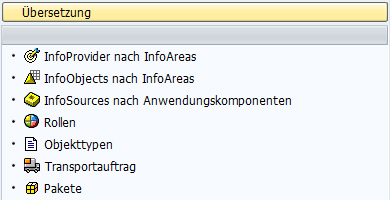
\includegraphics[width=0.5\textwidth]{files/Uebersetzung}
    \caption{Das Übersetzungsmenü}
    \label{pic:DWOverview}
\end{figure}
\item[Metadata Repository:] Das Metadata Repository basiert auf HTML und ermöglicht einen zentralen Zugriff auf Informationen von Metadaten-Objekten. Zu diesen Metadaten gehören zum Beispiel wichtige Eigenschaften der Objekte und die Verknüpfungen mit anderen Objekten.
\end{description}




